%! Author = lili
%! Date = 4/27/26


\section*{Vorlesung 1 (11.04.2025), ergänzt durch Skript}
\bluenote{Fehlkalkulationen durch unzureichende Modelle bzw. fehlende Parameter werden oft als Zufall gesehen. Wir versuchen Modelle so zu wählen, dass sie möglichst einfach sind.}
\begin{figure}[H]
    \centering
    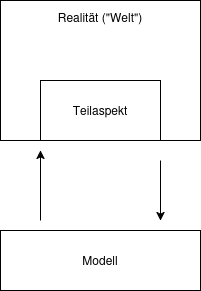
\includegraphics[width=0.3\textwidth]{images/model.png}
    \caption{}
    \label{fig:model}
\end{figure}

\subsection*{Lernziele}
\begin{itemize}
    \item modellieren einfacher Zufallsexperimente
    \item \gls{wraum} kennen und verwenden
    \item \Gls{gleichverteilung} kennen und erkennen
\end{itemize}

\subsection*{Begriffe}
\begin{defi}
    \textbf{\Gls{elementarereignis} \glssymbol{elementarereignis}} \\
    Möglicher Ausgang eines Zufallsexperiments. \\
    Es ist üblich, für Elementarereignisse den kleinen griechischen Buchstaben \glssymbol{elementarereignis} (omega) zu verwenden.
    Davon weichen wir in konkreten Situationen manchmal ab.
    So schreiben wir zum Beispiel auch $k$, wenn das Elementarereignis eine natürliche Zahl ist, oder $x$, wenn es
    eine reelle Zahl ist.
\end{defi}
\begin{bsp}
    \begin{itemize}
        \item Würfeln: $\glssymbol{elementarereignis} = 3$ (3 gewürfelt)
        \item Zeitmessung: $\glssymbol{elementarereignis} = 100$ (Sec)
    \end{itemize}
\end{bsp}

\begin{defi}
    \textbf{\Gls{eraum}} $\glssymbol{eraum}$ \\
    Die Menge aller Elementarereignisse $\glssymbol{eraum}  \neq \emptyset$ ist die Menge aller möglichen Ausgänge
    eines Zufallsexperiments. \\
    Ein Ereignisraum ist also zunächst einmal einfach eine nichtleere Menge.  \\
    Für einen Ereignisraum verwenden immer den großen griechischen Buchstaben $\glssymbol{eraum}$ (Omega). Wenn wir
    mehrere Ereignisräume benötigen, so schreiben wir
    $\glssymbol{eraum}, \tilde {\glssymbol{eraum}}, \glssymbol{eraum}_1, \glssymbol{eraum}_2, \dots$ usw.
\end{defi}
\begin{bsp}
    \begin{itemize}
        \item \textbf{Wuerfeln:}  $\glssymbol{eraum}  = \{1,\dots.,6\}$ oder $\glssymbol{eraum}  = \{ wuerfelsymbole \}$ \\
        Die Modellierung durch Würfelsymbole zeigt, daß es beim Modellieren wichtig ist anzugeben,
        welche Interpretation unsere Kodierung der Elementarereignisse haben soll. Man soll daher
        stets einen Satz der Art
        \begin{center}
            ``Dabei bedeutet $\glssymbol{elementarereignis} = wuerfelsymbol1$, dass der Würfel eine Eins zeigt''
        \end{center}
        schreiben, wenn man einen Ereignisraum angibt.
        \item \textbf{Zeitmessung:} $\glssymbol{eraum}  = [0, \infty)$ ist grundsätzlich eine sinnvolle Wahl, wenn wir das Messen einer
        zufälligen Zeit modellieren wollen. Sofern Zusatzinformationen vorliegen, können wir natürlich
        ein kleineres Intervall wählen.
        \bluenote{Siehe die Klammernnotation, die bedeutet die Null ist drin, aber infinity nicht (oder umgekehrt)}
    \end{itemize}
\end{bsp}
Häufig interessiert uns gar nicht der exakte Ausgang eines Zufallsexperiments, sondern nur, ob der
Ausgang eine bestimmte Eigenschaft hat: Haben wir eine gerade Zahl gewürfelt? Ist die gemessene
Zeit kürzer als eine Minute? Wir fassen also jene Elementarereignisse zusammen, die die gewünschte
Eigenschaft haben. Dies führt zur folgenden Definition.

\begin{defi} \textbf{Ereignis} $A$ \\
(Messbare) Teilmenge des Ereignisraums $A \subseteq \glssymbol{eraum}  $(
$A = \emptyset, A = \glssymbol{eraum} )$ sind zulässig) \\
Sprechweise: $\glssymbol{elementarereignis} \in A$ bedeutet ``A ist eingetroffen''
\end{defi}
Im Fall, dass der Ereignisraum $\glssymbol{eraum} \subseteq \rz^n$ weder eine endliche noch eine abzählbar unendliche
Menge ist, beschränken wir uns auf Ereignisse, die Intervalle oder bekannte geometrische Figuren wie Dreieck,
Rechteck oder Kugel sind.
Auch abzählbare Schnitte oder Vereinigungen solcher Objekte sind zulässig, sowie deren abzählbare Schnitte oder Vereinigungen.
Und so weiter.
Diese Einschränkung erlaubt es uns, Fragen der mathematischen Maß- und Integrationstheorie zu vermeiden.

\begin{bem}
    \begin{itemize}
        \item Ein Ereignis $A \subseteq \glssymbol{eraum}$ ist also ein (meßbares) Element der Potenzmenge $\glssymbol{potenz}(\glssymbol{eraum})$
        von $\glssymbol{eraum}$, das heißt, $A \in \glssymbol{potenz}(\glssymbol{eraum})$.
        \item Ist $\glssymbol{elementarereignis} \in \glssymbol{eraum}$ ein Elementarereignis, so ist die
        einelementige Menge $\{\glssymbol{elementarereignis}\} \in \glssymbol{potenz}(\glssymbol{eraum})$
        ein Ereignis in $\glssymbol{eraum}$.
    \end{itemize}
\end{bem}

\begin{bsp}
    \begin{itemize}
        \item \textbf{Würfeln} einer geraden Zahl: \[A = \{2,4,6\}, \quad \glssymbol{elementarereignis} = 4 \Rightarrow \glssymbol{elementarereignis} \in A\] Wir sagen: ``gerade Zahl gewürfelt''
        \item \textbf{Zeitmessung:} $A = [100, 200] \subset \glssymbol{eraum}  = [0,\infty)$
    \end{itemize}
\end{bsp}


\section{Vorgehen beim Modellieren}
\bluenote{Beim geeigneten $\glssymbol{eraum} $ können Modelle sich bereits unterscheiden. Bspw. Münzwurf: Man kann ``k'', ``z'' nahmen oder ``Kopf'', ``Zahl''. Das sind verschiedenen $\glssymbol{eraum} $, aber beide wären passend.}
\begin{itemize}
    \item Finden des geeigneten $\glssymbol{eraum} $
    \item Ereignisse müssen \gls{ws} zugeordnet bekommen
    \begin{enumerate}
        \item \textbf{Möglichkeit}: \gls{ws} für $\glssymbol{eraum} $ abzählbar
    \end{enumerate}
\end{itemize} \vskip 14pt \orangenote{Wenn sie abzählbar sagt, meint sie sowohl endlich als auch abzählbar unendlich.}

\begin{defi}
    \textbf{Zähldichte / \acrfull{wfk}} \\
    Sei $\glssymbol{eraum}  \neq \emptyset$ eine abzählbare Menge.
    \begin{itemize}
        \item[(i)] Eine Abbildung $\glssymbol{wfk} : \glssymbol{eraum}  \rightarrow [0,1]$ heißt mit \[
                                                                                                         \underbrace{\sum_{\glssymbol{elementarereignis} \in \glssymbol{eraum} } \glssymbol{wfk} (\glssymbol{elementarereignis}) = 1}_{\text{\txo{Normierung}}}
        \] \underline{Zähldichte / \gls{wfk}} auf $\glssymbol{eraum} $. \\
        \bluenote{Die Reihe (Normierung) muss 1 sein und konvergieren.} \bluenote{Wenn man max abzählbar hat, dann sind die Wahrscheinlichkeiten einfach teile der Summe (Normierung) und daher ist das einfach.}
        \item[(ii)] Die \gls{ws} $\pe(A)$ einer Ereignisses $A \subseteq \glssymbol{eraum} $ ist bei gegebener \gls{wfk} $\glssymbol{wfk}$ definiert durch
        \[ \pe(A)\coloneqq \sum_{w \in A} \glssymbol{wfk}(\glssymbol{elementarereignis})\]   \bluenote{Was hat die Potenzmenge von Omega damit zu tun?}
        \noindent $\pe$ heißt \gls{wmaß} und liegt immer zwischen Null und 1
        \begin{itemize}
            \item[] \textit{Konvention}: $\pe(\emptyset) = 0$
        \end{itemize}
    \end{itemize}
    \begin{bem}
        \[0 \leq \pe \leq 1, \quad \forall A \subseteq \glssymbol{eraum}  \quad \txo{\underbrace{(\forall A \in \glssymbol{potenz}(\glssymbol{eraum} )) }_{\glssymbol{potenz}(\glssymbol{eraum} ) \text{Potenzmenge von } \glssymbol{eraum} }} \]
        $\pe$ ist eine Abb.
        \[
            \pe: \glssymbol{potenz}(\glssymbol{eraum} ) \rightarrow [0,1] \quad  \text{ mit }  \pe(\emptyset) = 0, \quad  \pe(\glssymbol{eraum} ) = 1
        \]
    \end{bem}
\end{defi}

\begin{lem} \textbf{Eigenschaften des Wahrscheinlichkeitsmaßes für abzählbare Ereignisräume} \\
    Sei $\glssymbol{eraum} \neq \emptyset$ eine abzählbare Menge und $\glssymbol{wmaß}$ ein Wahrscheinlichkeitsmaß auf $\glssymbol{eraum}$.
Dann gelten:
    \begin{itemize}
        \item $0 \leq \pe (A) \leq 1$ für alle $A \leq \glssymbol{potenz}(\glssymbol{eraum})$
        \item $\pe(\epmtyset) = 0$
        \item $\pe(\glssymbol{eraum}) = 1$
    \end{itemize}
    % TODO \paragraph{Beweis} im Skript
\end{lem}

\begin{defi}
    \textbf{\gls{wraum}} \\
    $\underbrace{\glssymbol{wraum}}_{\txo{(\glssymbol{eraum} , \glssymbol{wfk})}}$ heißt \underline{\gls{wraum}}.
    \begin{bem}
        % TODO noch die längere aus dem Skript dazu holen
        Für $\glssymbol{eraum} $ abzählbar: $\glssymbol{wfk}$ legt $\pe$ eindeutig und umgekehrt!
        \[P(A)=\sum_{\glssymbol{elementarereignis} \in A} \glssymbol{wfk} (\glssymbol{elementarereignis}) \quad \forall A \in \glssymbol{potenz}(\glssymbol{eraum} )\]
        \[\glssymbol{wfk} (\glssymbol{elementarereignis}) = \pe(\underbrace{\{\glssymbol{elementarereignis}\}}_{\txo{\text{1-elementige Menge}}}) \quad \forall \glssymbol{elementarereignis} \in \glssymbol{eraum} \]
    \end{bem}
\end{defi} %
\begin{bsp}
    \textbf{Einmal Würfeln} \\
    $\glssymbol{eraum}  = \{1,..,6\}, \quad A = \{6\} \text{ (sechs gewürfel)}, \quad B = \{2,4,6\}$ (gerade Zahl). \\
    \textcolor{Orchid}{Dabei beudeute $\glssymbol{elementarereignis} = k$, dass der Würfel $k$ Augen hat.} \bluenote{In Hausaufgaben zu jedem Omega hinzuschreiben, was es bedeutet! ``Dabei beudeute $\glssymbol{elementarereignis} = k$, dass \dots''}
    Wie wählen wir $\glssymbol{wfk}$?
    \begin{itemize}
        \item[(a)] \textbf{fairer Würfel}: \bluenote{Ein ebener Würfel ist ein ``fairer Würfel'', weil alle Seiten gleich Wahrscheinlich sind.}
        \[\glssymbol{wfk}(k) = const \  \forall k \in \glssymbol{eraum} \]
        \[\glssymbol{wfk} (k) \coloneqq \frac{1}{6} \text{(weil $\sum_{k=1} \glssymbol{wfk} (k) \overset{!}{=} 1$ )}\]
        $\pe(A) = \glssymbol{wfk}(a) = \frac{1}{6}, \quad \pe(B) \sum_{k \in \{2,4,6\}} \glssymbol{wfk}(k) = \frac{1}{6} \cdot \#B = \frac{3}{6} = \frac{1}{2}$
        \item[(b)] \textbf{gezinkter Würfel}: Seien
        \[\glssymbol{wfk}(1) = \frac{1}{2}, \glssymbol{wfk}(2) = \glssymbol{wfk}(3) = \glssymbol{wfk}(4) = \glssymbol{wfk}(5) = \frac{1}{12}, \glssymbol{wfk}(6)=\frac{1}{6}\]
        Probe: $\sum_{k=1}^6 \glssymbol{wfk}(k) \overset{!}{=} 1$ \bluenote{In der Klausur wenn bei einer Probe ein Fehler herauskommt, gerne hinschreiben man hat gemerkt da ist ein Fehler und wo der gewesen sein muss, besser als nichts hischreiben.}
    \end{itemize}
\end{bsp}
Wie wählen wir $\glssymbol{eraum} $ und $\glssymbol{wfk}$ (bzw. $\pe$)?
\begin{itemize}
    \item Frage der Erfahrung
    \item wichtiges Thema und Lernziel dieses Semester
\end{itemize}
\begin{bsp}
    \textbf{Zweimal würfeln mit fairem Würfel - Augensumme}
    \begin{enumerate}
        \item \textbf{Ansatz}: $\glssymbol{eraum} _1 = \{1,\dots,6\}^2 = \{(i,j): i,j \in \{1,\dots,6\}\}$  \\
        \textcolor{Orchid}{ Für $\glssymbol{elementarereignis} = (i,j) \in \glssymbol{eraum} _1$ bedeutet $i$ die Augenzahl des ersten Würfels und $j$ jene des zweiten Würfels.} \\
        Aus Symmetriegründen wählen wir $\glssymbol{wfk}_1(\glssymbol{elementarereignis})$ konstant, also  \[\glssymbol{wfk}_1(\glssymbol{elementarereignis}) = \frac{1}{|\glssymbol{eraum} _1|} = \frac{1}{36} \quad \forall \glssymbol{elementarereignis} \in \glssymbol{eraum} _1\]
        \underline{ $A^{(1)}_k \leq \glssymbol{eraum} _1$}: Augensumme ist $k$ \\
        \underline{ Für $k \leq 1$ oder $k \leq 13$:} \[A^{(1)}_k = \emptyset \Rightarrow \pe_1 (A^{(1)}_k) = 0\]
        \underline{Für $k = \{2,,12\}$:}
        \[\pe_1 (A^{(1)}_2) = \pe_1 (\{(1,1)\}) = \glssymbol{wfk}_1((1,1)) = \frac{1}{36}\]
        \[\pe_1 (A^{(1)}_3) = \pe_1 (\{(1,2), (2,1)\}) = \glssymbol{wfk}_1((1,2)) + \glssymbol{wfk}_1((2,1)) = \frac{2}{36}\]
        usw\dots Es wird immer eines mehr \\
        \begin{tabular}{c|ccccccccccccc}
            $k$ & 2 & 3 & 4 & 5 & 6 & 7 & 8 & 9 & 10 & 11 & 12 \\
            $\pe_1 (A^{(1)}_k)$ & $\frac{1}{36}$ & $\frac{2}{36}$ & $\frac{3}{36}$ & $\frac{4}{36}$ & $\frac{5}{36}$
            & $\frac{6}{36}$
            & $\frac{5}{36}$
            & $\frac{4}{36}$
            & $\frac{3}{36}$
            & $\frac{2}{36}$
            & $\frac{1}{36}$
        \end{tabular} \\
        Probe: \[\sum_{k=2}^{12} mathbb{P}_1 (A^{(1)}_k) = 1\]
        \item \textbf{Ansatz}: ``Wir beachten die Reihenfolge beim Würfeln nicht'' \\
        $\glssymbol{eraum} _2 = \{(i,j) \in \glssymbol{eraum} _1: i \leq j\}$ \\
        \textcolor{Orchid}{ Dabei bedeute $\glssymbol{elementarereignis} =(i,j)$, dass sowohl i alas auch j gewürfelt wurden. } \\
        Finde $\glssymbol{wfk}_2$! \\
        \begin{itemize}
            \item[(1)] \underline{$i \le j$:} $1 \times i$ und $1 \times j$ gewürfelt
            \[\glssymbol{wfk}_2((i,j)) = \glssymbol{wfk}_1((i,j)) + \glssymbol{wfk}_1((j,i)) = \frac{2}{36}\]
            \item[(2)] \underline{$i = j$:} $2 \times i $ gewürfelt
            \[\glssymbol{wfk}_2((i,i)) = \frac{1}{36}\]
        \end{itemize}
        Probe machen!
        \[A^{(2)}_k = \{(i,j) \in \glssymbol{eraum} _2: i+j = k\}\]
        Exemplische Ausrechnung:
        \[\pe_2(A^{(2)}_4) = \glssymbol{wfk}_2((1,3)) + \glssymbol{wfk}_2((2,2)) = \frac{2}{36} + \frac{1}{36} = \frac{3}{26}\]
        \item \textbf{Ansatz}: $\glssymbol{eraum} _3$ = \{2,3,..,12\} \\
        Finde $\glssymbol{wfk}_3$?
        $\rightarrow$ Verwende Tabelle aus dem 1. Ansatz, denn $\glssymbol{wfk}_3(k) = \pe(A^{(1)}_k)$ :  \\
        \begin{tabular}{c|ccccccccccccc}
            $k$ & 2 & 3 & 4 & 5 & 6 & 7 & 8 & 9 & 10 & 11 & 12 \\
            \textcolor{Aquamarine}{$\glssymbol{wfk}_3(k)$} & $\frac{1}{36}$ & $\frac{2}{36}$ & $\frac{3}{36}$
            & $\frac{4}{36}$
            & $\frac{5}{36}$
            & $\frac{6}{36}$
            & $\frac{5}{36}$
            & $\frac{4}{36}$
            & $\frac{3}{36}$
            & $\frac{2}{36}$
            & $\frac{1}{36}$
        \end{tabular}
    \end{enumerate}%

\end{bsp}
\bluenote{Man hat beim Modellieren immer die Wahl. Und mann muss aufpassen wie man es macht. }
\begin{bsp}
    \textbf{Reißzwecke ``würfeln'' - Symmetrieüberlegungen helfen nicht} \\
    $\glssymbol{eraum}  = \{R, S\}$ (R auf Kopf, S auf Seite) \\
    Definition: $\glssymbol{wfk}(S) > \glssymbol{wfk}(R)$ \\
    10.000 Würfe; 4213 R \\
    Möchte $\glssymbol{wfk}(R) \approx \frac{4213}{10.000} = 0,4213$ (relative Häufigkeit) \\ \textcolor{Orchid}{-> Gesetz der gr. Zahlen  \\ -> Statistik}
\end{bsp}
Take-Home message: Wann immer möglich, modelliere so, dass $\glssymbol{wfk}(\glssymbol{elementarereignis}) = const \forall \glssymbol{elementarereignis} \in \glssymbol{eraum} $ (erfordert Symmetrieargumente)

\begin{defi}
    \textbf{Gleichverteilung} \\
    Sei $\glssymbol{eraum}  \neq \emptyset$ eine endl. Menge, d.h. $0 < \#\glssymbol{eraum}  < \infty$. Gilt $\glssymbol{wfk}(\glssymbol{elementarereignis}) = \glssymbol{wfk}(\tilde{\glssymbol{elementarereignis}}) \quad  \forall \glssymbol{elementarereignis}, \tilde{\glssymbol{elementarereignis}} \in \glssymbol{eraum} $ d.h. die \gls{wfk} $\glssymbol{wfk}$ ist konstant, so heißen die wfkt mu und das zugehörige wmaß P die \underline{Gleichverteilung auf $\glssymbol{eraum} $}
\end{defi}
\begin{lem}
    Sei $\glssymbol{wfk}$ die Gleichverteilung auf $\glssymbol{eraum} $. Dann gelten:
    \begin{itemize}
        \item[(a)] $\glssymbol{wfk}(\glssymbol{elementarereignis}) = \frac{1}{\#\glssymbol{eraum} } \quad \forall \glssymbol{elementarereignis} \in \glssymbol{eraum} $
        \item[(b)] $\pe(A) = \frac{\#A}{\#\glssymbol{eraum} } \forall A \in \pe(\glssymbol{eraum} )$ \txo{($\forall A \subseteq \glssymbol{eraum} $)}
    \end{itemize}

    \paragraph{Beweis.}
    \begin{itemize}
        \item[(a)] \(1 = \sum_{\glssymbol{elementarereignis} \in \glssymbol{eraum} } \glssymbol{wfk}(\glssymbol{elementarereignis}) = \) \footnote{Wir dürfen annehmen, dass ein $c \in [0,1]$ existiert mit $\glssymbol{wfk}(\glssymbol{elementarereignis}) = c \quad \forall \glssymbol{elementarereignis} \in \glssymbol{eraum} $}$\ c \cdot \# \glssymbol{eraum}  \Rightarrow c = \frac{1}{\#\glssymbol{eraum} }$
        \item[(b)] $\pe(A) = \sum_{\glssymbol{elementarereignis} \in A } \glssymbol{wfk}(\glssymbol{elementarereignis}) \overset{(a)}{=} \frac{\#A}{\# \glssymbol{eraum} }$ \\
        \txo{$\pe(A)$ ist die Anzahl der günstigen Ausgänge, geteilt durch die Anzahl aller möglichen Ausgänge} \\

    \end{itemize}
\end{lem}
\begin{bem}
    Im Fall der Gleichverteilung reduziert sich das Berechnen von WS auf Abzählprobleme. \\ \bluenote{Mathe 1}
\end{bem}
\begin{bem} % aus Skript
    \textbf{Keine Gleichverteilung, wenn der Ereignisraum nicht endlich ist} \\
    Warum müssen wir voraussetzen, dass $\# \glssymbol{eraum} < \infty $?
    Nehmen wir an, es gäbe eine Gleichverteilung $\glssymbol{elementarereignis}$ auf einer abzählbar unendlichen Menge
    $\glssymbol{eraum}$.
    Wir können der Einfachheit halber annehmen, dass $\glssymbol{eraum}$ die Menge
    der natürlichen Zahlen $\mathbb{N}$ ist.
    Dann gibt es also ein $c \in [0, 1]$ mit
    \[
        1 = \sum^{\infty}_{k = 1} \glssymbol{elementarereignis}(k)    = c \cdot \# \mathbb{N}
    \]
    Nun gibt es zwei Fälle.
    Entweder, $c = 0$.
    Dann erhalten wir den Widerspruch $1 = 0$.
    Andernfalls, wenn $c > 0$ gilt, erhalten wir ebenfalls einen Widerspruch, nämlich $1 = \infty$.
    Folglich kann es auf einer nicht endlichen Menge keine Gleichverteilung geben
\end{bem}
\begin{bsp}
    \textbf{Gleichverteilung}
    \begin{itemize}
        \item $1 \times $ Werfen einer fairen Münze: $\glssymbol{eraum}  = \{K,Z\}, \glssymbol{wfk}(\glssymbol{elementarereignis}) = \frac{1}{2} \forall \glssymbol{elementarereignis} \in \glssymbol{eraum} $
        \item $1 \times$ Würfeln oder  $2 \times$ Würfeln mit fairem Würfel
    \end{itemize}
\end{bsp}
\begin{bsp}
    \textbf{KEINE Gleichverteilung}
    \begin{itemize}
        \item Augensumme beim wiederholten Würfeln
        \item Werfen einer Reißzwecke
    \end{itemize}
\end{bsp}
\newpage
